\documentclass[a4paper]{article}

\usepackage{ReportTemplate}

\usepackage{setspace}
\usepackage{amsmath}
\usepackage[hidelinks]{hyperref}
\usepackage[ruled,lined,commentsnumbered]{algorithm2e}

\title{Project 1:语音端点检测}
\name{邱一航}
\studentid{520030910155}

\begin{document}

\maketitle

\setcounter{section}{-1}
\section{说明}

本文为AI2651《智能语音识别》课程的第一次大作业报告。

\section{基于线性分类器和语音时域特征的简单语音端点检测算法}

\subsection{数据预处理及特征提取}

\subsubsection{音频预处理}

对原始的输入音频,笔者尝试了如下的两种不同预处理方式。(记原始音频为$x[n]$,预处理后的音频为$\tilde{x}[n]$)

\begin{itemize}
    \item \textbf{平滑。}将当前离散时间点附近的一段矩形窗内的所有信号取平均值作为当前时间点的信号。记矩形窗长度为奇数$2L+1$,则该过程用如下公式表示:
    \begin{align*}
        \tilde{x}[n]=\frac{1}{2L+1}\sum_{k=n-L}^{n+L} x[k]
    \end{align*}
    \item \textbf{预加重。}查阅相关资料\cite{Pre-emphasis}后得知,该方法能够去除口唇辐射的影响,增强语音的高频部分及高频分辨率。预加重处理可用如下公式表示:(其中预加重系数$\alpha$的一般取值范围是$\alpha\in[0.9,1]$)
    \begin{align*}
        \tilde{x}[n]=x[n] - \alpha x[n-1]
    \end{align*}
\end{itemize}

在附件中程序($\mathtt{task1.py}$或$\mathtt{task1.ipynb}$)的Hyperpatameter定义部分,设置了两个变量决定是否使用上述两种预处理方式。

\begin{lstlisting}[language=python]
# For frame segmentation:
Smooth = False
#Pre-emphasis: 
Emph = True
a = .9
\end{lstlisting}

其中,$\mathtt{Smooth}$和$\mathtt{Emph}$为$\mathtt{True}$时表示使用对应的方法进行预处理,$a$是预加重系数。

\subsubsection{帧分割}

笔者在程序中编写了$\mathtt{Frame\_Seg}$函数用于将原始音频切割为帧。

本次大作业中,笔者并未过多研究不同帧大小和帧偏移对语音端点检测效果的影响,仅做了几次实验对比检测效果,最终采用了效果较好的0.032秒和0.008秒的默认值。

\subsubsection{特征提取}

对预处理后的数据,笔者进行了以下两种特征的提取。

\begin{itemize}
    \item \textbf{短时能量,}即单个帧内所有采样点上信号的能量和。记$N$为帧的长度,用$s$表示当前帧,则短时能量可用如下公式表述:
    \begin{equation*}
        E(s) = \sum_{k=0}^{N-1}(s[k])^2
    \end{equation*}
    
    \item \textbf{过零率,}即每一帧中采样后信号跨越零点的次数。记$N$为帧的长度,用$s$表示当前帧,则过零率可用如下公式表示:
    \begin{align*}
        Z(s) & = \frac{1}{2}\left[\sum_{k=1}^{N-1} \big|\mathtt{sgn}(s[k])\big|-\big|\mathtt{sgn}(s[k-1])\big|\right] \\
        & \text{其中\ }\mathtt{sgn}(x)=\left\{\begin{array}{ll}
            1, & x\geq0 \\
            0, & x<0
        \end{array}\right.
    \end{align*}
\end{itemize}

\subsection{算法描述}

下图(见下页中的图\ref{fig1})是一段音频短时能量和过零率的可视化。蓝色折线为短时能量,红色折线为过零率,黑色折线为语音标记,值为1表示是语音,为0表示不是语音。

\begin{figure}[htb]
  \hspace{-3.6em}
  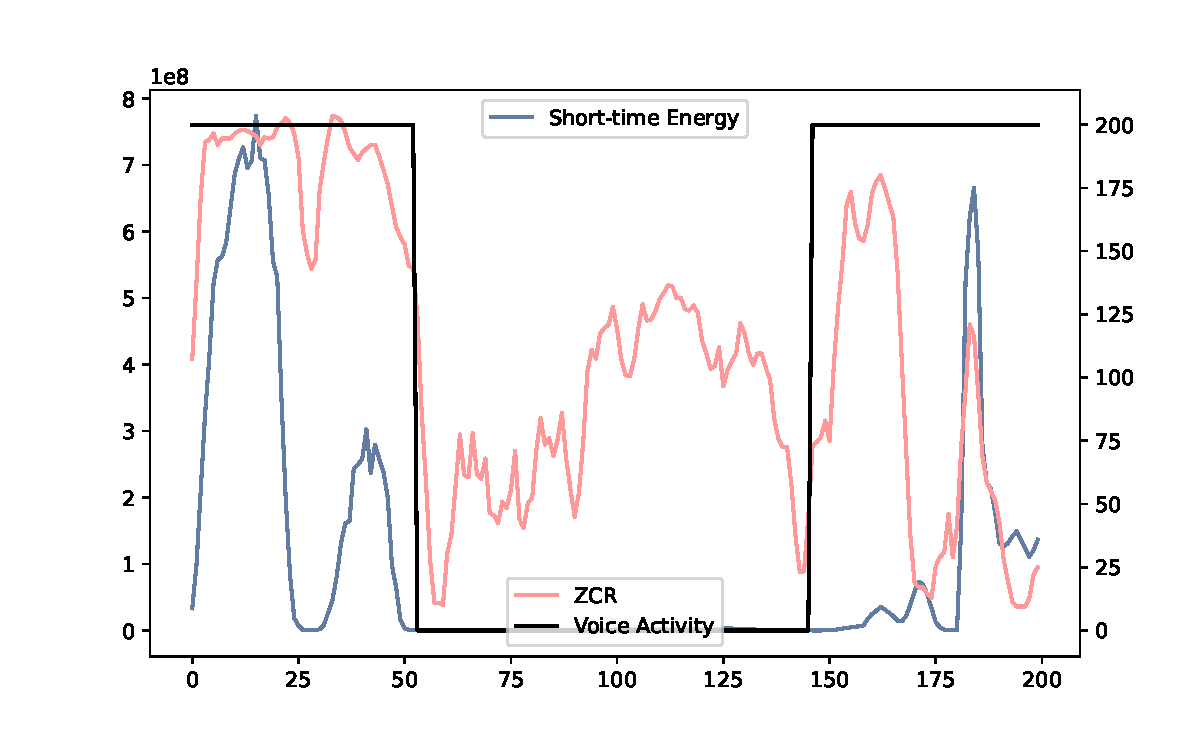
\includegraphics[scale=0.5]{figs/voice_example.pdf}
  \caption{Visualization of Short-time Energy and ZCR}
  \label{fig1}
\end{figure}

结合课程中已讲述的语音特征等知识,观察被标记为“语音”的音频段落与标记为“非语音”的段落的短时能量与过零率,可以发现:

\begin{itemize}
    \item 语音部分可以近似看作“浊音”和“清音”的组合,且浊音与清音一般是互相紧邻出现的。
    \item 浊音部分短时能量较高,且浊音开始部分会迅速达到一个较高的峰值,随后逐渐下降。浊音的过零率不一定非常高,因此用短时能量判断更准确。
    \item 清音部分的短时能量较低,但过零率非常高。
\end{itemize}

因此,基于\textbf{1.1}中所提取的两种特征,笔者分别进行如下处理:

\begin{itemize}
    \item 使用\textbf{短时能量}判断浊音。为了能取得更好的效果,笔者采用了\textbf{双门限法}判断,即当短时能量超过高阈值时,认为接下来的帧都属于浊音;当短时能量下降到低阈值时,认为浊音结束。这样处理可以更精确地判断浊音,同时又可以将浊音的尾部(短时能量相对较低的部分)正确地判断为浊音。
    
    \item 使用\textbf{过零率}判断清音。这里笔者尝试了两种不同方式:
    \begin{itemize}
        \item 从所有已经获得的浊音两端出发,根据过零率判断当前帧是否为清音,认为过零率高于一定阈值即为清音。最终的所有语音帧即所有清音帧与浊音帧。
        \item 对过零率也使用\textbf{双门限法},单独查找清音。随后查找浊音与清音段落之间短时能量大于能量低阈值且过零率大于过零率低阈值的过渡段,标记为语音。
    \end{itemize}
    
\end{itemize}

第一种方法(对短时能量使用双门限法判断浊音,再在浊音附近用过零率单门限判断清音)的伪代码如下。

\begin{algorithm}
        \caption{短时能量双门限、过零率单门限法}
        \setstretch{1.1}
        \SetKwProg{function}{Function}{}{end}
        \SetKwProg{subroutine}{Subroutine}{}{end}
        \SetKwProg{procedure}{Procedure}{}{end}
        \SetKwInOut{return}{Return}
        \SetKwProg{repeat}{repeat}{}{end}
	    \function{VAD$(S, \alpha, \beta, \gamma, \delta)$}
	    {
	        \tcp{$S$是所有帧的集合。$\alpha$和$\beta$分别是短时能量的高、低阈值;$\gamma$和$\delta$分别是过零率的高、低阈值。}
	        $pred\gets\left\{\text{非语音}\right\}_{s\in S}$\;
	        \tcp{$pred$标记每个帧是否为语音。}
	        \BlankLine
	        \BlankLine
	        \While{$s\in Ss$}
	        {
	            \While{$G(s)<\alpha$}{$s\gets$ $S$中的后一帧;}
	            \While{$G(s)\geq \beta$}
	            {
	                $pred[s]\gets \text{是语音}$\;
	                $s\gets$ $S$中的后一帧\;
	            }
            }
            \While{$s_0\in S$ s.t. $s_0$是语音}
            {
                $s\gets s_0$\;
                \While{$s$的过零率$\geq\gamma$}
                {
                $pred[s]\gets$是语音\;
                $s\gets$ $S$中的前一帧\;
                }
                $s\gets s_0$\;
                \While{$s$的过零率$\geq\gamma$}
                {
                $pred[s]\gets$是语音\;
                $s\gets$ $S$中的后一帧\;
                }
	        }
	        \return{$pred$}
	   }
    \end{algorithm}

第二种方法(对短时能量和过零率均使用双门限法,并对过渡段特殊处理)的伪代码如下。

\begin{algorithm}
        \caption{能量双门限、过零率单门限法}
        \setstretch{1.1}
        \SetKwProg{function}{Function}{}{end}
        \SetKwProg{subroutine}{Subroutine}{}{end}
        \SetKwProg{procedure}{Procedure}{}{end}
        \SetKwInOut{return}{Return}
        \SetKwProg{repeat}{repeat}{}{end}
        
        \subroutine{2-Th$(S,G,a,b,pred)$}
        {
            \tcp{双门限。}
            \tcp{$S$是所有帧的集合,$G$是短时能量或过零率的计算函数。$a$是高阈值,$b$是低阈值。$pred$标记了每个帧是否为语音。}
            \While{$s\in frames$}
	        {
	            \While{$G(s)<a$}{$s\gets$ $S$中的后一帧;}
	            \While{$G(s)\geq b$}
	            {
	                $pred[s]\gets \text{是语音}$\;
	                $s\gets$ $S$中的后一帧\;
	            }
            }
        }
        \BlankLine
        \BlankLine
	    \function{VAD$(S, \alpha, \beta, \gamma, \delta)$}
	    {
	        \tcp{$S$是等待识别语音端点的音频经切割后得到的帧集合。$\alpha$和$\beta$分别是短时能量的高阈值和低阈值;$\gamma$和$\delta$分别是过零率的高阈值和低阈值。}
	        $pred\gets\left\{\text{非语音}\right\}_{s\in S}$\;
	        \tcp{$pred$标记每个帧是否为语音。}
	        \BlankLine
	        \BlankLine
	        \textit{2-Th}($S,\text{短时能量},\alpha,\beta,pred)$\;
            \textit{2-Th}($S,$ZCR$,\gamma,\delta,pred)$\;
            \While{$s_0\in S$ s.t. $s_0$是语音}
            {
                $s\gets s_0$\;
                \While{$s$的短时能量$\geq\beta$且$s$的ZCR$\geq\delta$}
                {
                $pred[s]\gets$是语音\;
                $s\gets$ $S$中的前一帧\;
                }
                $s\gets s_0$\;
                \While{$s$的短时能量$\geq\beta$且$s$的ZCR$\geq\delta$}
                {
                $pred[s]\gets$是语音\;
                $s\gets$ $S$中的后一帧\;
                }
	        }
	        \return{$pred$}
	   }
    \end{algorithm}

以上算法中的阈值均可视为“硬阈值”,即不会随音频文件变化而变化。然而,考虑到不同的音频文件中,短时能量的平均值未必一致,因此笔者还尝试将音频所有帧的短时能量\textbf{归一化处理}后,再进行上述操作。即对每个音频文件切割后的帧集合$S$,做以下操作:

\vspace{-1em}
\begin{align*}
    \mu(S) & \triangleq \frac{1}{|S|}\sum_{s\in S}E(S) \\
    \sigma(S) & \triangleq \frac{1}{|S|}\sum_{s\in S}(E(S)-\mu)^2 \\
    \forall s\in S, \tilde{E}(s) &= \frac{E(s)-\mu(S)}{\sigma(S)} \\
\end{align*}

\vspace{-1em}
之后对$\tilde{E}(s)$用上述两种算法处理出语音端点。此时设置的各种阈值可视为“可变阈值”,对归一化前的短时能量而言是一个与能量的均值、方差相关的变量。

因此实际上笔者共设计了四种不同的算法。下将每个音频的短时能量归一化后使用算法1的方法称为“算法3”,短时能量归一化后使用算法2称为“算法4”。这四种算法在不同的数据预处理下的效果请见\textbf{1.3}。

\subsection{实验结果}

在不同的数据预处理(是否平滑、是否预加重)下,\textbf{1.2}中所提及的四种算法在开发集上的效果(AUC,ERR,ACC(准确率))如表\ref{tab1}所示。

由于每种方法都有各自的参数需要调节,下表中的结果均为各自方法下的最好效果;各种情况下的最佳参数在表\ref{tab2}中给出。

特别地,表中加粗的几种具有代表性的方法,其具体参数在附件中的程序文件中作为默认值存在。这几种代表性算法在测试集上的测试结果在task1文件夹中均有给出,其中$\mathtt{test\_label\_task.txt}$保存的是预加重后使用算法1的结果。

(\textbf{注}:由于使用平滑后效果普遍\textbf{更差}(AUC下降且ERR上升),因此并未对平滑且预加重原始数据的情况进行实验。)

\newpage

\begin{table}[th]
  \centering
  \begin{tabular}{ c c c c c}
    \toprule
    \textbf{方法} & \textbf{预处理} & \textbf{AUC} & \textbf{ERR} & \textbf{ACC} \\
    \midrule
    \textbf{算法1} & \textbf{无} & \textbf{0.8906} & \textbf{0.1242} & \textbf{0.8690} \\
    算法2 & 无 & 0.8897 & 0.1297 & 0.8479 \\
    \textbf{算法3} & \textbf{无} & \textbf{0.7525} & \textbf{0.3890} & \textbf{0.7283}\\
    算法4 & 无 & 0.7212 & 0.3803 & 0.7028\\
    \midrule
    算法1 & 平滑 & 0.8663 & 0.1858 & 0.8422\\
    算法2 & 平滑 & 0.8593 & 0.1901 & 0.8230\\
    算法3 & 平滑 & 0.7533 & 0.3906 & 0.7391\\
    算法4 & 平滑 & 0.7294 & 0.3952 & 0.7102\\
    \midrule
    \textbf{算法1} & \textbf{无} & \textbf{0.9012} & \textbf{0.1178} & \textbf{0.8782} \\
    算法2 & 预加重 & 0.8983 & 0.1216 & 0.8623\\
    算法3 & 预加重 & 0.7614 & 0.3778 & 0.7590\\
    算法4 & 预加重 & 0.7308 & 0.3695 & 0.7219\\
    \bottomrule
  \end{tabular}
  \vspace{0.5em}
  \centering \caption{基于语音时域特征的简单算法检测效果对比}
  \label{tab1}
\end{table}

\vspace{-1em}
注意表中加粗的仅为较有代表性且参数被保存的算法,并不一定是开发集上效果最佳的算法。

使用平滑预处理后,数据的过零率被改变了,因而不再能很好地通过过零率来判断清音的位置,导致几乎所有方法的AUC下降且ERR上升。

显然效果最佳的是使用预加重处理后的算法1(对短时能量使用双门限判断浊音,再在浊音附近的语音片段上利用过零率查找清音语音片段),该方法也作为附件中程序中的默认方法。三种加粗的代表性算法对应的参数如下表。

\begin{table}[th]
  \centering
  \begin{tabular}{ p{30pt} p{33pt} p{45pt} p{45pt} p{27pt} }
    \toprule
    \textbf{\ 方法} & \textbf{预处理} & \textbf{短时能量高阈值} & \textbf{短时能量低阈值} & \textbf{ZCR阈值} \\
    \midrule
    算法1 & \ \ \ 无 & 300000000 & 7500000 & 100 \\
    算法3 & \ \ \ 无 & 1.0 & 0.8 & 0.9 \\
    算法1 & 预加重 & 30000000 & 750000 & 1000 \\
    \bottomrule
  \end{tabular}
  \vspace{0.5em}
  \centering \caption{三种代表性方法的最佳参数}
  \label{tab2}
\end{table}

\section{基于统计模型分类器和语音频域特征的语音端点检测算法}

\subsection{数据预处理及特征提取}

\subsubsection{音频预处理}
    由\textbf{1.3}实验可见,\textbf{预加重}这一预处理方式使所有方法的效果都得到了增强,因此这里我们依然采用预加重作为预处理方式,公式如下。笔者选取的预加重系数$\alpha=0.9$。
    \begin{align*}
        \tilde{x}[n]=x[n] - \alpha x[n-1]
    \end{align*}
    
\subsubsection{帧切割}
    由于后续将要使用频域特征,为了保证不引入频率噪声,我们在帧分割时将直接切割获得的帧乘上窗函数,使每一帧的边缘较为“柔和平滑”。
    
    记原始音频为$x[n]$,切割得到的某一帧为$s[n]$,窗函数为$w[n]$,帧长度为$L$。则该过程即为
    \begin{equation*}
        \tilde{s}[n] = s[n]\cdot w[n]\ (n=0,1,...,L-1)
    \end{equation*}
    
    其中窗长(即$w[n]$的长度)与帧长度$L$需要完全一致。
    
    笔者在实验中选用了汉宁窗(Hanning Window),但在程序实现时也实现了使用其他窗进行边缘平滑的功能,详见附件中的程序$\mathtt{task2.ipynb}$和$\mathtt{task2.py}$。
    
    汉宁窗的时域和频域性质如图\ref{fig2}所示。
    
\begin{figure}[htb]
  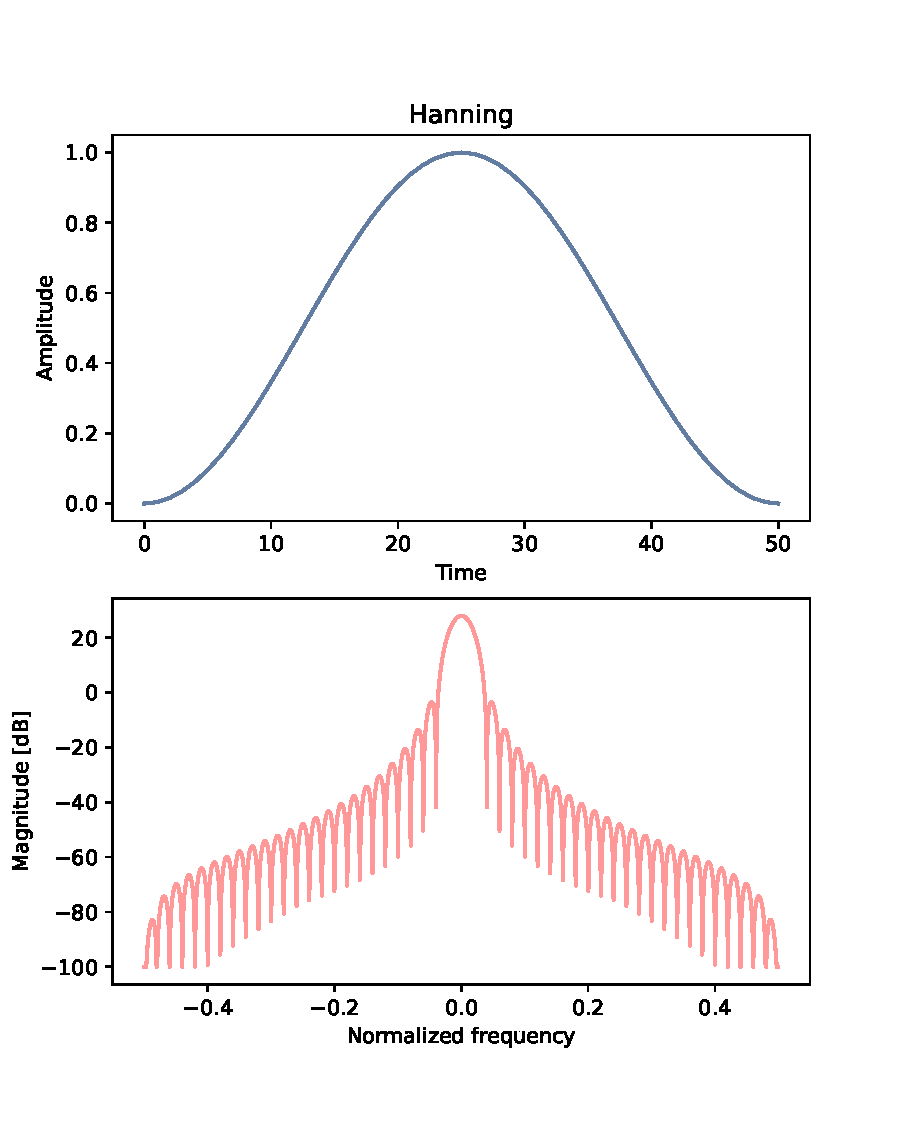
\includegraphics[scale=0.5]{figs/hanning.pdf}
  \caption{The Visualization of Hanning Window on Time Domain and Frequency Domain}
  \label{fig2}
\end{figure}

\subsubsection{频域特征提取}

笔者选用了MFCC(Mel-Frequency Cepstral Coefficients,梅尔滤波器倒谱系数)和FBank(Filter Bank)两种特征。实际上,前者是后者经过处理得到的,因此两者的本质实际上是一致的。具体的代码实现详见$\mathtt{task2.ipynb}$或$\mathtt{task2.py}$。

Mel滤波器是一系列(一般为40个)滤波器,滤波器通频上下限频率转化为梅尔后是等差数列。该滤波器组能很好地模拟人耳的听觉特性。

\subsection{算法描述}

    笔者基于MFCC和FBank两种频域特征,分别使用了神经网络(DNN)进行该部分实验。
    
    笔者在sklearn和pytorch上分别尝试实现了神经网络,不同之处在于笔者直接调用了前者提供的MLPClassifier,而在后者提供的平台上自己定义了神经网络及其训练。因此,实际上在该部分实验中,笔者一共实现了四个神经网络。它们的不同结构和训练方式如下。
    
    \subsubsection{神经网络结构描述}
    四个网络均为MLP,即多层感知器(最朴素的神经网络)。表格中给出了每一层的神经元个数。
    
    (注:“预设”指使用了sklearn预设的MLPClassifier;“自定义”指基于pytorch提供的nn.Module模块进行自定义网络构建。)
\begin{table}[th]
  \centering
  \begin{tabular}{ c c l}
    \toprule
    \textbf{基于特征} & \textbf{网络实现} & \textbf{结构} \\
    \midrule
    MFCC & 预设 & $12\to24\to12\to6\to4\to2$ \\
    FBank & 预设 & $40\to40\to20\to10\to4\to2$ \\
    MFCC & 自定义 & $12\to12\to4\to1$ \\
    FBank & 自定义 & $40\to10\to8\to4\to1$ \\
    \bottomrule
  \end{tabular}
  \vspace{0.5em}
  \centering \caption{神经网络结构说明}
  \label{tab3}
\end{table}
    
\subsubsection{神经网络训练方式}
    
    对前两个网络,由于笔者使用了预设的sklearn.neural\_network.MLPClassifier实现,训练时\textbf{只需要调用}.fit(features, labels)函数即可,其中features是输入的特征(由整个训练集的特征组成),labels是features对应的分类(此处即为0/1,即语音或非语音)。
    
    对后两个网络,笔者将网络最终的输出pred(含义是语音的概率)与训练集上的标签label做二分类交叉熵loss(BCE Loss),试图让两者尽可能接近(即非语音的输出接近0,语音帧的输出接近1)。但后续实验表明自定义网络在这种训练下效果不佳,具体分析详见\textbf{2.3}。
    
    值得一提的是,对pytorch上自定义的网络,如果loss函数仅考虑让网络的输出与训练集上的标签结果尽可能接近,很有可能会得到网络输出大部分为1或大部分为0的情况,因为该情况下loss函数也达到了一个极小值。
    
    因此,笔者在后两个网络上也尝试了一些其他方式想要避免这种情况的发生,如引入\textbf{负采样}来让训练集中语音段落和非语音段落的出现概率更加接近(具体尝试详见$\mathtt{task2\_neg.ipynb}$)。此外,笔者还试图在loss函数中加入如下的正则项来避免输出全为0或全为1的情况(该正则项在输出的平均值接近0或1时会很大,从而避免输出中0或1出现概率过高的情况)。
    
    \vspace{-1em}
    \begin{align*}
        Reg(pred) &= \mathtt{tan}\left(\left(\mathtt{mean}(pred)-\frac{1}{2}\right)\pi\right). 
    \end{align*}
    
    其中$\mathtt{mean}(\cdot)$为求平均值。则loss函数变为:
    
    \vspace{-1em}
    \begin{align*}
        Loss(pred,label) &= BCELoss(pred,label) \\
        &+ \gamma Reg(pred)
    \end{align*}
        
    但后续实验证明这两种尝试的效果依然非常糟糕,远远不如sklearn预设的神经网络中的预设训练方式。因此,笔者最终只使用基于sklearn预设的两个神经网络在test集上生成语音端点识别结果。
    
    \subsubsection{神经网络参数说明}
    
    神经网络训练采用梯度下降。对于基于sklearn预设实现的神经网络,需要设定最大训练轮数max\_iter。对于基于pytorch自定义建构的神经网络,需要设置训练轮数。笔者在程序中的Hyperparameter定义部分设置了变量Training\_epoch用以设置神经网络的训练轮数。
    
    此外,训练时需要设置学习率。笔者在程序中的Hyperparameter定义部分设置了Learning\_rate变量用以全局调节学习率。
    
    此外,神经网络输入向量的形状实际上取决于MFCC和FBank的参数,即梅尔滤波器的数目和对FBank进行DCT(离散余弦变换)生成MFCC时保留的频率个数。这两个参数会决定神经网络的输入向量的形状。
    
    笔者在程序中设定的默认值也是前人使用MFCC和FBank参数的常用值,即40个梅尔滤波器,在DCT后的FBank中保留13个频率。
    
    特别地,对使用\textbf{2.2.2}中正则项的网络,存在用于调节正则项在loss中占比大小的超参数$\gamma$。
    
    以上参数都在程序$\mathtt{task2.ipynb}$和$\mathtt{task2.py}$的Hyperparameter定义部分被定义,它们的默认值如下。
    
    \begin{lstlisting}[language=python]
    # For MFCC and FBank.
    Num_filters = 40
    Minmax_Ceps = (1,13)
    # For Machine Learning Traning.
    Training_epoch = 100
    Learning_rate = 0.01
    # Regularization on Loss.
    gamma = 0.1
\end{lstlisting}
    
    

\subsection{实验结果}

基于MFCC、FBank两种特征,基于sklearn的预设和使用pytorch自定义构建的四个神经网络训练完毕后,在开发集上的检测效果如表\ref{tab4}。

\begin{table}[th]
  \centering
  \begin{tabular}{ c c c c c }
    \toprule
    \textbf{神经网络} & \textbf{特殊处理} & \textbf{AUC} & \textbf{ERR} & \textbf{ACC}\\
    \midrule
    MFCC,预设 & 无 & 0.9433 & 0.1187 & 0.8947\\
    \textbf{FBank,预设} & \textbf{无} & \textbf{0.9778} & \textbf{0.0652} & \textbf{0.8991}\\
    \midrule
    MFCC,自定义 & 无 & 0.6951 & 0.3373 & 0.7165\\
    FBank,自定义 & 无 & 0.7941 & 0.4022 & 0.6704\\
    \midrule
    MFCC,自定义 & 负采样 & 0.5832 & 0.4347 & 0.8051\\
    FBank,自定义 & 负采样 & 0.6620 & 0.3989 & 0.8136\\
    \midrule
    MFCC,自定义 & 正则项 & 0.6230 & 0.3272 & 0.7123\\
    FBank,自定义 & 正则项 & 0.6941 & 0.4193 & 0.7931\\
    \bottomrule
  \end{tabular}
  \vspace{0.5em}
  \centering \caption{基于语音频域特征的神经网络检测效果对比}
  \label{tab4}
\end{table}

可以看出,基于sklearn预设实现的神经网络效果远远好于笔者使用pytorch定义的神经网络。导致这一结果的可能原因有:

\begin{itemize}
    \item 笔者使用的loss函数虽然能提升预测是否为语音(输出0/1)的准确性,但是从程序的中间输出来看,网络的输出中经常出现“大量0”和“大量1”的情况,虽然该结果的“预测准确率”确实升高了,但是AUC相对较少,实际上效果变差。因此,笔者设计的loss与实际目标并不完全相符。
    \item 训练轮数不足。由于自定义实现网络debug完成后,距离截止时限只有一天,为了能得出结果,笔者将训练轮数下调至20。20轮训练并不足以完成我们所定义的神经网络的训练(尤其是对引入负采样的神经网络)。因此,我们自定义的神经网络预测效果较差。
\end{itemize}

此外可以发现,无论是基于sklearn预设还是基于pytorch的自定义网络,基于FBank的网络预测效果均高于基于MFCC的网络。这是由于MFCC实际上是FBank经非线性变换并舍弃部分信息得到的,其信息含量不如FBank,因此预测效果会稍微劣于基于FBank的神经网络。

值得一体的是,基于sklearn预设的两个网络在开发集上效果非常良好,它们极高的AUC和极低的ERR反而让我有些担忧存在过拟合的问题。但是神经网络是在训练集上训练得到的且在开发集上只测试了一次,且ACC并没有高得离谱,因此我认为这一惊人的结果应该不是过拟合的情况。

\section{鸣谢}

完成本大作业的过程中,就\textbf{2}中神经网络的训练与loss正则项的设计问题,笔者与\textbf{王崇华}、\textbf{季弋琨}两位同学进行了讨论。在此特别感谢两位同学的帮助。

\begin{thebibliography}{}

\bibitem[1]{Pre-emphasis} 语音信号的预加重处理和加窗处理,CSDN, https://blog.csdn.

net/ziyuzhao123/article/details/12004603

\end{thebibliography}

\end{document}